\documentclass[12pt]{article}
\usepackage[a4paper, landscape]{geometry}
\usepackage[poster]{tcolorbox}
\pagestyle{empty}

% Font
\usepackage{fontspec}
\newfontfamily\arial{Arial}
\setmainfont{Arial Bold}

% Graphics
\usepackage{svg}

% Document
\begin{document}
\begin{tcbposter}[
    coverage = {
      spread,
      interior style={white},
    },
    poster = {showframe=true, columns=4, rows=5},
    boxes = {colback=white, colframe=white}
  ]
  \posterbox{name=chemicalname, column=1, span=3}{
    \resizebox{16cm}{!}{Hydrogen peroxide}\\[5mm]
    \resizebox{7cm}{!}{CAS: 7722-84-1}
  }
  \posterbox{name=logo, column=4, span=1}{
    \includesvg{logos/thylabs}
  }
  \posterbox{name=NFPA704, row=3, column=4}{
    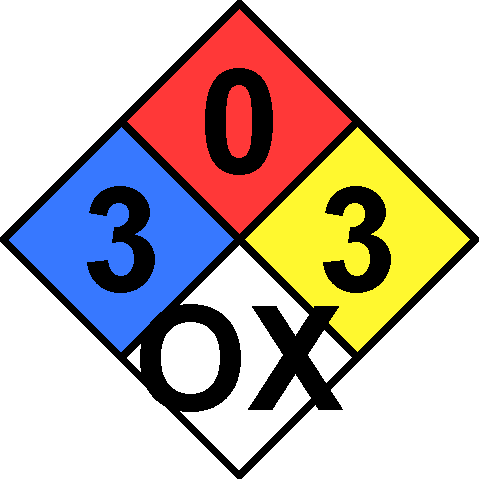
\includegraphics[scale=0.75]{parts/NFPA_test784.pdf}
  }
\end{tcbposter}
\end{document}
